% Seminar 9: Machine learning for time series
% Time Series Analysis -- Bachelor's programmes Economic Informatics and Economic Cybernetics, Bucharest University of Economic Studies
% GENERATED by latex/build_seminar9.py -- edit the generator, not this file.
% Student version by default; the instructor version is the *_solutions.tex wrapper.
\makeatletter\@ifundefined{ifsolutions}{\expandafter\newif\csname ifsolutions\endcsname}{}\makeatother

\newcommand{\coursename}{Time Series Analysis}
% Preambul comun TSA -- Serii de timp / Time Series Analysis (Beamer, 16:9)
% Același design ca MFM și SFM (preluat din SFM, 5 octombrie 2026). Înainte de % Preambul comun TSA -- Serii de timp / Time Series Analysis (Beamer, 16:9)
% Același design ca MFM și SFM (preluat din SFM, 5 octombrie 2026). Înainte de % Preambul comun TSA -- Serii de timp / Time Series Analysis (Beamer, 16:9)
% Același design ca MFM și SFM (preluat din SFM, 5 octombrie 2026). Înainte de \input{../../latex/preamble} se definește
%   \newcommand{\coursename}{Time Series Analysis}      (EN)
%   \newcommand{\coursename}{Serii de timp}       (RO)  și  \def\tsalang{ro}
% Fișierele .tex se află în EN/Courses, EN/Seminars, RO/Cursuri, RO/Seminarii (două niveluri sub rădăcină).
% Deck-urile sînt generate de latex/build_chapterN.py / build_seminarN.py (vezi latex/tsa_build.py).

\documentclass[9pt, aspectratio=169, t]{beamer}
\providecommand{\coursename}{Time Series Analysis}

% Ensure content fits on slides
\setbeamersize{text margin left=8mm, text margin right=8mm}
% Smaller institute font (title page)
\setbeamerfont{institute}{size=\footnotesize}

%=============================================================================
% THEME AND STYLE CONFIGURATION
%=============================================================================
\usetheme{default}
% Using default theme for clean header/footer control

% Color Palette (matching Redispatch PDF)
\definecolor{MainBlue}{RGB}{26, 58, 110}
\definecolor{AccentBlue}{RGB}{26, 58, 110}
\definecolor{IDAred}{RGB}{205, 0, 0}
\definecolor{DarkGray}{RGB}{51, 51, 51}
\definecolor{MediumGray}{RGB}{128, 128, 128}
\definecolor{LightGray}{RGB}{248, 248, 248}
\definecolor{VeryLightGray}{RGB}{235, 235, 235}
\definecolor{KeynoteGray}{RGB}{218, 218, 218}
\definecolor{SectionGray}{RGB}{120, 120, 120}
\definecolor{FooterGray}{RGB}{100, 100, 100}
\definecolor{Crimson}{RGB}{220, 53, 69}
\definecolor{Forest}{RGB}{46, 125, 50}
\definecolor{Amber}{RGB}{181, 133, 63}
\definecolor{Orange}{RGB}{230, 126, 34}
\definecolor{Purple}{RGB}{142, 68, 173}

% Gradient background (exact Keynote 315° gradient: white to RGB 218,218,218)
\setbeamertemplate{background}{%
    \begin{tikzpicture}[remember picture, overlay]
        \shade[shading=axis, shading angle=315,
        top color=white, bottom color=KeynoteGray]
        (current page.south west) rectangle (current page.north east);
    \end{tikzpicture}%
}
% Fallback solid color for compatibility
\setbeamercolor{background canvas}{bg=}

\setbeamercolor{palette primary}{bg=MainBlue, fg=white}
\setbeamercolor{palette secondary}{bg=MainBlue!85, fg=white}
\setbeamercolor{palette tertiary}{bg=MainBlue!70, fg=white}
\setbeamercolor{structure}{fg=MainBlue}
\setbeamercolor{title}{fg=IDAred}
\setbeamercolor{frametitle}{fg=IDAred, bg=}
\setbeamercolor{block title}{bg=MainBlue, fg=white}
\setbeamercolor{block body}{bg=VeryLightGray, fg=DarkGray}
\setbeamercolor{block title alerted}{bg=Crimson, fg=white}
\setbeamercolor{block body alerted}{bg=Crimson!8, fg=DarkGray}
\setbeamercolor{block title example}{bg=Forest, fg=white}
\setbeamercolor{block body example}{bg=Forest!8, fg=DarkGray}
\setbeamercolor{item}{fg=MainBlue}

% Footer colors (override Madrid theme blue)
\setbeamercolor{author in head/foot}{fg=FooterGray, bg=}
\setbeamercolor{title in head/foot}{fg=FooterGray, bg=}
\setbeamercolor{date in head/foot}{fg=FooterGray, bg=}
\setbeamercolor{section in head/foot}{fg=FooterGray, bg=}
\setbeamercolor{subsection in head/foot}{fg=FooterGray, bg=}

% Bullet styles (apply everywhere including blocks)
\setbeamertemplate{itemize item}{\color{MainBlue}$\boxdot$}
\setbeamertemplate{itemize subitem}{\color{MainBlue}$\blacktriangleright$}
\setbeamertemplate{itemize subsubitem}{\color{MainBlue}\tiny$\bullet$}
\setbeamertemplate{itemize/enumerate body begin}{\normalsize}
\setbeamertemplate{itemize/enumerate subbody begin}{\normalsize}

% Item spacing - compact style
\setlength{\leftmargini}{10pt}       % Level 1: minimal indent
\setlength{\leftmarginii}{10pt}      % Level 2: minimal additional indent
% Compact list spacing (zero extra space before/after lists in blocks)
\makeatletter
\def\@listi{\leftmargin\leftmargini \topsep 0pt \parsep 0pt \itemsep 0pt}
\def\@listii{\leftmargin\leftmarginii \topsep 0pt \parsep 0pt \itemsep 0pt}
\makeatother

\setbeamertemplate{navigation symbols}{}

%=============================================================================
% CUSTOM HEADLINE
%=============================================================================
\setbeamertemplate{headline}{%
    \vskip10pt%
    \hbox to \paperwidth{%
        \hskip0.5cm%
        {\small\color{FooterGray}\renewcommand{\hyperlink}[2]{##2}\insertsectionhead}%
        \hfill%
        \textcolor{FooterGray}{\small\insertframenumber}%
        \hskip0.5cm%
    }%
    \vskip4pt%
    {\color{FooterGray}\hrule height 0.4pt}%
}

%=============================================================================
% CUSTOM FOOTER
%=============================================================================
\usepackage{fontawesome5}

\setbeamertemplate{footline}{%
    {\color{FooterGray}\hrule height 0.4pt}%
    \vskip4pt%
    \hbox to \paperwidth{%
        \hskip0.5cm%
        \textcolor{FooterGray}{\small\coursename}%
        \hfill%
        \raisebox{-0.1em}{%
            \begin{tikzpicture}[x=0.08em, y=0.08em, line width=0.4pt]
                \draw[FooterGray] (0,3) -- (1,4) -- (2,3.5) -- (3,5) -- (4,4) -- (5,6) -- (6,5.5) -- (7,4) -- (8,5) -- (9,7) -- (10,6) -- (11,5) -- (12,6.5) -- (13,8) -- (14,7) -- (15,6) -- (16,7.5) -- (17,9) -- (18,8) -- (19,7) -- (20,8.5) -- (21,10) -- (22,9) -- (23,8) -- (24,9.5);
            \end{tikzpicture}%
        }%
        \hskip0.5cm%
    }%
    \vskip6pt%
}

%=============================================================================
% PACKAGES
%=============================================================================
\usepackage[utf8]{inputenc}
\DeclareUnicodeCharacter{03B1}{\ensuremath{\alpha}}
\usepackage[T1]{fontenc}
\usepackage{amsmath, amssymb, amsthm}
\usepackage{mathtools}
\usepackage{bm}
\usepackage{tikz}
\usetikzlibrary{arrows.meta, positioning, shapes, calc, decorations.pathreplacing, shadings}
\usepackage{booktabs}
\usepackage{multirow}
\usepackage{array}
\usepackage{graphicx}
\usepackage{animate}
\usepackage{hyperref}
\usepackage{colortbl}
\usepackage{listings}
\lstset{language=Python, basicstyle=\ttfamily\scriptsize, keywordstyle=\color{MainBlue}\bfseries,
  commentstyle=\color{Forest}, stringstyle=\color{Crimson}, breaklines=true,
  frame=none, backgroundcolor=\color{VeryLightGray}, xleftmargin=2mm}
\hypersetup{colorlinks=true, linkcolor=MainBlue, urlcolor=MainBlue}
\graphicspath{{../../logos/}{../../charts/}{../../photos/}}
\usepackage{xcolor}
\hfuzz=2pt  % Suppress tiny overfull warnings (<2pt)
\vfuzz=2pt  % Suppress tiny vertical overfull warnings (<2pt)
% \mathrm in the sans-serif family of the slides (beamer resets \mathrm to the serif family at \begin{document};
% this hook runs after beamer's, so WN, Var, RMSE, ... in formulas match the surrounding text)
% Bold vectors and matrices in the same sans-serif family: \mathbf{A} in sans bold (beamer's own \mathbf came out in
% medium weight), and the bold upright Greek capitals of \boldsymbol / \bm (\bSigma, \bPhi, \boldsymbol{\Theta}) in
% cmss bold: bm.sty fixes its "boldoperators" font when it is loaded (serif cmbx), before beamer switches the
% operators to cmss, so it is reset here.
\AtBeginDocument{%
  \SetMathAlphabet{\mathrm}{normal}{\encodingdefault}{\sfdefault}{\mddefault}{n}%
  \SetMathAlphabet{\mathrm}{bold}{\encodingdefault}{\sfdefault}{bx}{n}%
  \SetMathAlphabet{\mathbf}{normal}{\encodingdefault}{\sfdefault}{bx}{n}%
  \SetMathAlphabet{\mathbf}{bold}{\encodingdefault}{\sfdefault}{bx}{n}%
  \SetSymbolFont{boldoperators}{normal}{OT1}{cmss}{bx}{n}%
  \SetSymbolFont{boldoperators}{bold}{OT1}{cmss}{bx}{n}}

%=============================================================================
% QUANTLET COMMANDS
%   \quantlet{<displayed name>}{<url>}       (generic, compatible with the older TSA decks)
%   \tsaquantlet{Ch_05}{TSA_ch5_garch}       -> https://github.com/danpele/Time-Series-Analysis/tree/main/Quantlets/Ch_05/TSA_ch5_garch
%   \qlurl{<folder>} is defined per chapter by the generator (Quantlets/Ch_NN/<folder>)
%=============================================================================
\newcommand{\tsarepo}{https://github.com/danpele/Time-Series-Analysis}
\newcommand{\tsaqlbase}{https://github.com/danpele/Time-Series-Analysis/tree/main/Quantlets}
\newcommand{\quantlet}[2]{%
    \hfill\href{#2}{%
        \raisebox{-0.15em}{
\includegraphics[height=0.7em]{ql_logo.png}}%
        \textcolor{MainBlue}{\tiny\ #1}%
    }%
}
\newcommand{\tsaquantlet}[2]{\quantlet{\detokenize{#2}}{\tsaqlbase/#1/#2}}

%=============================================================================
% NOTEBOOKS (Google Colab)
%   \colaburl{notebooks/EN/chapter5_seminar_notebook.ipynb} -> the Colab link of a file in the TSA repo
%   \nb: the chapter notebook (each seminar deck redefines it with \renewcommand)
%=============================================================================
\newcommand{\colaburl}[1]{https://colab.research.google.com/github/danpele/Time-Series-Analysis/blob/main/#1}
\newcommand{\nb}{https://colab.research.google.com/github/danpele/Time-Series-Analysis/tree/main/notebooks/EN}
\newcommand{\nbname}{notebooks/EN}

%=============================================================================
% SLIDE HELPERS (used by the generators; the same as in MFM)
%=============================================================================
% local font size for list bodies (the preamble forces \normalsize)
\newcommand{\itemsize}[1]{\setbeamertemplate{itemize/enumerate body begin}{#1}\setbeamertemplate{itemize/enumerate subbody begin}{#1}}
\newcommand{\intitle}[1]{{\hypersetup{urlcolor=white}#1}}   % white links inside coloured title bars
\newcommand{\imgcap}[1]{{\scriptsize #1}\\[0.5mm]}          % caption under a photo
\newcommand{\imgcredit}[2]{{\tiny\color{FooterGray}\href{#1}{#2}}}   % image credit: source URL, author/licence
\newcommand{\aiprompt}[1]{{\ttfamily\color{MainBlue}#1}}     % a prompt to an AI assistant

%=============================================================================
% SEMINARS: student version by default; the instructor wrapper *_solutions.tex sets \solutionstrue
%=============================================================================
\makeatletter\@ifundefined{ifsolutions}{\expandafter\newif\csname ifsolutions\endcsname}{}\makeatother
\newcommand{\solonly}[1]{\ifsolutions #1\fi}
\newcommand{\propsub}{\ifsolutions\else\framesubtitle{\ifdefined\tsalang Rezolvarea se discută la seminar\else Solution discussed in class\fi}\fi}

%=============================================================================
% APPENDIX AND CHAPTER LINKS (latex/appendix_links.py writes the calls; it also re-declares these
% macros before \begin{document}, so the decks compile with or without this preamble block)
%=============================================================================
\providecommand{\tsaapplink}[3]{\hypertarget{#2}{}\hyperlink{#1}{\beamergotobutton{#3}}}
\providecommand{\tsaappback}[2]{\begin{tikzpicture}[remember picture,overlay]\node[anchor=south east] at ([xshift=-3mm,yshift=7mm]current page.south east){\hyperlink{#1}{\beamerreturnbutton{#2}}};\end{tikzpicture}}
\providecommand{\tsachlink}[2]{\href{#1}{#2}}
\providecommand{\tsachlinkt}[2]{\href{#1}{\usebeamercolor[fg]{frametitle}#2}}

%=============================================================================
% QUANTINAR COMMAND: link către un curs Quantinar (subiecte avansate)
%=============================================================================
\newcommand{\quantinar}[2]{%
    \href{#2}{%
        \raisebox{-0.15em}{
\includegraphics[height=0.8em]{qr_logo.png}}%
        \textcolor{MainBlue}{\scriptsize\ #1}%
    }%
}

%=============================================================================
% CUSTOM TITLE PAGE
%=============================================================================
\defbeamertemplate*{title page}{hybrid}[1][]
{
    \vspace{0.2cm}
    % Logos row - top header (with clickable links)
    \begin{center}
        \href{https://www.ase.ro}{
\includegraphics[height=1.0cm]{ase_logo.png}}\hspace{0.3cm}%
        \href{https://theida.net}{
\includegraphics[height=1.0cm]{ida_logo.png}}\hspace{0.3cm}%
        \href{https://blockchain-research-center.com}{
\includegraphics[height=1.0cm]{brc_logo.png}}\hspace{0.3cm}%
        \href{https://www.ai4efin.ase.ro}{
\includegraphics[height=1.0cm]{ai4efin_logo.png}}\hspace{0.3cm}%
        \href{https://ipe.ro/new}{
\includegraphics[height=1.0cm]{acad_logo.png}}\hspace{0.3cm}%
        \href{https://www.digital-finance-msca.com}{
\includegraphics[height=1.0cm]{msca_logo.png}}%
    \end{center}

    \vspace{0.6cm}

    % Main title with Q logos on sides (with clickable links)
    \begin{center}
        \begin{minipage}{0.1\textwidth}
            \centering
            \href{https://quantlet.com}{
\includegraphics[height=1.1cm]{ql_logo.png}}
        \end{minipage}%
        \begin{minipage}{0.78\textwidth}
            \centering
            {\LARGE\bfseries\usebeamercolor[fg]{title}\inserttitle}

            \vspace{0.3cm}

            {\usebeamerfont{subtitle}\usebeamercolor[fg]{title}\insertsubtitle}
        \end{minipage}%
        \begin{minipage}{0.1\textwidth}
            \centering
            \href{https://quantinar.com}{
\includegraphics[height=1.1cm]{qr_logo.png}}
        \end{minipage}
    \end{center}

    \vspace{0.6cm}

    % Authors (left aligned)
    \hspace{0.5cm}{\usebeamerfont{author}\insertauthor}

    \vspace{0.3cm}

    % Institute/Affiliations (left aligned)
    \hspace{0.5cm}\begin{minipage}[t]{0.9\textwidth}
        \raggedright\small\insertinstitute
    \end{minipage}
}

%=============================================================================
% THEOREM ENVIRONMENTS
%=============================================================================
\theoremstyle{definition}
\setbeamertemplate{theorems}[numbered]
\ifdefined\tsalang
\newtheorem{defn}{Definiție}
\newtheorem{thm}{Teoremă}
\newtheorem{prop}{Propoziție}
\newtheorem{rmk}{Observație}
\else
\newtheorem{defn}{Definition}
\newtheorem{thm}{Theorem}
\newtheorem{prop}{Proposition}
\newtheorem{rmk}{Remark}
\fi

%=============================================================================
% CENTRED MINIPAGE (no extra vertical space)
%=============================================================================
\newenvironment{cminipage}[1]{%
    \par\noindent\hfill\begin{minipage}{#1}\ignorespaces
}{%
    \end{minipage}\hfill\null\par
}

%=============================================================================
% CUSTOM COMMANDS
%=============================================================================
\newcommand{\E}{\mathbb{E}}
\newcommand{\Var}{\text{Var}}
\newcommand{\Cov}{\text{Cov}}
\newcommand{\Corr}{\text{Corr}}
\newcommand{\R}{\mathbb{R}}
\newcommand{\N}{\mathbb{N}}
\newcommand{\Z}{\mathbb{Z}}
\newcommand{\B}{\mathbf{B}}
\newcommand{\imark}{\textcolor{MainBlue}{\textbullet}}
\newcommand{\RMSE}{\text{RMSE}}
\newcommand{\MAE}{\text{MAE}}
\newcommand{\MAPE}{\text{MAPE}}

% Boldface vector/matrix commands (VAR, VECM, state space; also used by the older TSA decks)
\newcommand{\bY}{\mathbf{Y}}
\newcommand{\bX}{\mathbf{X}}
\newcommand{\bA}{\mathbf{A}}
\newcommand{\bB}{\mathbf{B}}
\newcommand{\bepsilon}{\boldsymbol{\varepsilon}}
\newcommand{\bSigma}{\boldsymbol{\Sigma}}
\newcommand{\bPhi}{\boldsymbol{\Phi}}
\newcommand{\bGamma}{\boldsymbol{\Gamma}}
\newcommand{\bPi}{\boldsymbol{\Pi}}
\newcommand{\bc}{\mathbf{c}}
\newcommand{\balpha}{\boldsymbol{\alpha}}
\newcommand{\bbeta}{\boldsymbol{\beta}}
\newcommand{\bvarepsilon}{\boldsymbol{\varepsilon}}

% Legacy seminar marks (older TSA seminar decks)
\newcommand{\correct}{\textcolor{Forest}{\checkmark}}
\newcommand{\incorrect}{\textcolor{Crimson}{\texttimes}}
 se definește
%   \newcommand{\coursename}{Time Series Analysis}      (EN)
%   \newcommand{\coursename}{Serii de timp}       (RO)  și  \def\tsalang{ro}
% Fișierele .tex se află în EN/Courses, EN/Seminars, RO/Cursuri, RO/Seminarii (două niveluri sub rădăcină).
% Deck-urile sînt generate de latex/build_chapterN.py / build_seminarN.py (vezi latex/tsa_build.py).

\documentclass[9pt, aspectratio=169, t]{beamer}
\providecommand{\coursename}{Time Series Analysis}

% Ensure content fits on slides
\setbeamersize{text margin left=8mm, text margin right=8mm}
% Smaller institute font (title page)
\setbeamerfont{institute}{size=\footnotesize}

%=============================================================================
% THEME AND STYLE CONFIGURATION
%=============================================================================
\usetheme{default}
% Using default theme for clean header/footer control

% Color Palette (matching Redispatch PDF)
\definecolor{MainBlue}{RGB}{26, 58, 110}
\definecolor{AccentBlue}{RGB}{26, 58, 110}
\definecolor{IDAred}{RGB}{205, 0, 0}
\definecolor{DarkGray}{RGB}{51, 51, 51}
\definecolor{MediumGray}{RGB}{128, 128, 128}
\definecolor{LightGray}{RGB}{248, 248, 248}
\definecolor{VeryLightGray}{RGB}{235, 235, 235}
\definecolor{KeynoteGray}{RGB}{218, 218, 218}
\definecolor{SectionGray}{RGB}{120, 120, 120}
\definecolor{FooterGray}{RGB}{100, 100, 100}
\definecolor{Crimson}{RGB}{220, 53, 69}
\definecolor{Forest}{RGB}{46, 125, 50}
\definecolor{Amber}{RGB}{181, 133, 63}
\definecolor{Orange}{RGB}{230, 126, 34}
\definecolor{Purple}{RGB}{142, 68, 173}

% Gradient background (exact Keynote 315° gradient: white to RGB 218,218,218)
\setbeamertemplate{background}{%
    \begin{tikzpicture}[remember picture, overlay]
        \shade[shading=axis, shading angle=315,
        top color=white, bottom color=KeynoteGray]
        (current page.south west) rectangle (current page.north east);
    \end{tikzpicture}%
}
% Fallback solid color for compatibility
\setbeamercolor{background canvas}{bg=}

\setbeamercolor{palette primary}{bg=MainBlue, fg=white}
\setbeamercolor{palette secondary}{bg=MainBlue!85, fg=white}
\setbeamercolor{palette tertiary}{bg=MainBlue!70, fg=white}
\setbeamercolor{structure}{fg=MainBlue}
\setbeamercolor{title}{fg=IDAred}
\setbeamercolor{frametitle}{fg=IDAred, bg=}
\setbeamercolor{block title}{bg=MainBlue, fg=white}
\setbeamercolor{block body}{bg=VeryLightGray, fg=DarkGray}
\setbeamercolor{block title alerted}{bg=Crimson, fg=white}
\setbeamercolor{block body alerted}{bg=Crimson!8, fg=DarkGray}
\setbeamercolor{block title example}{bg=Forest, fg=white}
\setbeamercolor{block body example}{bg=Forest!8, fg=DarkGray}
\setbeamercolor{item}{fg=MainBlue}

% Footer colors (override Madrid theme blue)
\setbeamercolor{author in head/foot}{fg=FooterGray, bg=}
\setbeamercolor{title in head/foot}{fg=FooterGray, bg=}
\setbeamercolor{date in head/foot}{fg=FooterGray, bg=}
\setbeamercolor{section in head/foot}{fg=FooterGray, bg=}
\setbeamercolor{subsection in head/foot}{fg=FooterGray, bg=}

% Bullet styles (apply everywhere including blocks)
\setbeamertemplate{itemize item}{\color{MainBlue}$\boxdot$}
\setbeamertemplate{itemize subitem}{\color{MainBlue}$\blacktriangleright$}
\setbeamertemplate{itemize subsubitem}{\color{MainBlue}\tiny$\bullet$}
\setbeamertemplate{itemize/enumerate body begin}{\normalsize}
\setbeamertemplate{itemize/enumerate subbody begin}{\normalsize}

% Item spacing - compact style
\setlength{\leftmargini}{10pt}       % Level 1: minimal indent
\setlength{\leftmarginii}{10pt}      % Level 2: minimal additional indent
% Compact list spacing (zero extra space before/after lists in blocks)
\makeatletter
\def\@listi{\leftmargin\leftmargini \topsep 0pt \parsep 0pt \itemsep 0pt}
\def\@listii{\leftmargin\leftmarginii \topsep 0pt \parsep 0pt \itemsep 0pt}
\makeatother

\setbeamertemplate{navigation symbols}{}

%=============================================================================
% CUSTOM HEADLINE
%=============================================================================
\setbeamertemplate{headline}{%
    \vskip10pt%
    \hbox to \paperwidth{%
        \hskip0.5cm%
        {\small\color{FooterGray}\renewcommand{\hyperlink}[2]{##2}\insertsectionhead}%
        \hfill%
        \textcolor{FooterGray}{\small\insertframenumber}%
        \hskip0.5cm%
    }%
    \vskip4pt%
    {\color{FooterGray}\hrule height 0.4pt}%
}

%=============================================================================
% CUSTOM FOOTER
%=============================================================================
\usepackage{fontawesome5}

\setbeamertemplate{footline}{%
    {\color{FooterGray}\hrule height 0.4pt}%
    \vskip4pt%
    \hbox to \paperwidth{%
        \hskip0.5cm%
        \textcolor{FooterGray}{\small\coursename}%
        \hfill%
        \raisebox{-0.1em}{%
            \begin{tikzpicture}[x=0.08em, y=0.08em, line width=0.4pt]
                \draw[FooterGray] (0,3) -- (1,4) -- (2,3.5) -- (3,5) -- (4,4) -- (5,6) -- (6,5.5) -- (7,4) -- (8,5) -- (9,7) -- (10,6) -- (11,5) -- (12,6.5) -- (13,8) -- (14,7) -- (15,6) -- (16,7.5) -- (17,9) -- (18,8) -- (19,7) -- (20,8.5) -- (21,10) -- (22,9) -- (23,8) -- (24,9.5);
            \end{tikzpicture}%
        }%
        \hskip0.5cm%
    }%
    \vskip6pt%
}

%=============================================================================
% PACKAGES
%=============================================================================
\usepackage[utf8]{inputenc}
\DeclareUnicodeCharacter{03B1}{\ensuremath{\alpha}}
\usepackage[T1]{fontenc}
\usepackage{amsmath, amssymb, amsthm}
\usepackage{mathtools}
\usepackage{bm}
\usepackage{tikz}
\usetikzlibrary{arrows.meta, positioning, shapes, calc, decorations.pathreplacing, shadings}
\usepackage{booktabs}
\usepackage{multirow}
\usepackage{array}
\usepackage{graphicx}
\usepackage{animate}
\usepackage{hyperref}
\usepackage{colortbl}
\usepackage{listings}
\lstset{language=Python, basicstyle=\ttfamily\scriptsize, keywordstyle=\color{MainBlue}\bfseries,
  commentstyle=\color{Forest}, stringstyle=\color{Crimson}, breaklines=true,
  frame=none, backgroundcolor=\color{VeryLightGray}, xleftmargin=2mm}
\hypersetup{colorlinks=true, linkcolor=MainBlue, urlcolor=MainBlue}
\graphicspath{{../../logos/}{../../charts/}{../../photos/}}
\usepackage{xcolor}
\hfuzz=2pt  % Suppress tiny overfull warnings (<2pt)
\vfuzz=2pt  % Suppress tiny vertical overfull warnings (<2pt)
% \mathrm in the sans-serif family of the slides (beamer resets \mathrm to the serif family at \begin{document};
% this hook runs after beamer's, so WN, Var, RMSE, ... in formulas match the surrounding text)
% Bold vectors and matrices in the same sans-serif family: \mathbf{A} in sans bold (beamer's own \mathbf came out in
% medium weight), and the bold upright Greek capitals of \boldsymbol / \bm (\bSigma, \bPhi, \boldsymbol{\Theta}) in
% cmss bold: bm.sty fixes its "boldoperators" font when it is loaded (serif cmbx), before beamer switches the
% operators to cmss, so it is reset here.
\AtBeginDocument{%
  \SetMathAlphabet{\mathrm}{normal}{\encodingdefault}{\sfdefault}{\mddefault}{n}%
  \SetMathAlphabet{\mathrm}{bold}{\encodingdefault}{\sfdefault}{bx}{n}%
  \SetMathAlphabet{\mathbf}{normal}{\encodingdefault}{\sfdefault}{bx}{n}%
  \SetMathAlphabet{\mathbf}{bold}{\encodingdefault}{\sfdefault}{bx}{n}%
  \SetSymbolFont{boldoperators}{normal}{OT1}{cmss}{bx}{n}%
  \SetSymbolFont{boldoperators}{bold}{OT1}{cmss}{bx}{n}}

%=============================================================================
% QUANTLET COMMANDS
%   \quantlet{<displayed name>}{<url>}       (generic, compatible with the older TSA decks)
%   \tsaquantlet{Ch_05}{TSA_ch5_garch}       -> https://github.com/danpele/Time-Series-Analysis/tree/main/Quantlets/Ch_05/TSA_ch5_garch
%   \qlurl{<folder>} is defined per chapter by the generator (Quantlets/Ch_NN/<folder>)
%=============================================================================
\newcommand{\tsarepo}{https://github.com/danpele/Time-Series-Analysis}
\newcommand{\tsaqlbase}{https://github.com/danpele/Time-Series-Analysis/tree/main/Quantlets}
\newcommand{\quantlet}[2]{%
    \hfill\href{#2}{%
        \raisebox{-0.15em}{
\includegraphics[height=0.7em]{ql_logo.png}}%
        \textcolor{MainBlue}{\tiny\ #1}%
    }%
}
\newcommand{\tsaquantlet}[2]{\quantlet{\detokenize{#2}}{\tsaqlbase/#1/#2}}

%=============================================================================
% NOTEBOOKS (Google Colab)
%   \colaburl{notebooks/EN/chapter5_seminar_notebook.ipynb} -> the Colab link of a file in the TSA repo
%   \nb: the chapter notebook (each seminar deck redefines it with \renewcommand)
%=============================================================================
\newcommand{\colaburl}[1]{https://colab.research.google.com/github/danpele/Time-Series-Analysis/blob/main/#1}
\newcommand{\nb}{https://colab.research.google.com/github/danpele/Time-Series-Analysis/tree/main/notebooks/EN}
\newcommand{\nbname}{notebooks/EN}

%=============================================================================
% SLIDE HELPERS (used by the generators; the same as in MFM)
%=============================================================================
% local font size for list bodies (the preamble forces \normalsize)
\newcommand{\itemsize}[1]{\setbeamertemplate{itemize/enumerate body begin}{#1}\setbeamertemplate{itemize/enumerate subbody begin}{#1}}
\newcommand{\intitle}[1]{{\hypersetup{urlcolor=white}#1}}   % white links inside coloured title bars
\newcommand{\imgcap}[1]{{\scriptsize #1}\\[0.5mm]}          % caption under a photo
\newcommand{\imgcredit}[2]{{\tiny\color{FooterGray}\href{#1}{#2}}}   % image credit: source URL, author/licence
\newcommand{\aiprompt}[1]{{\ttfamily\color{MainBlue}#1}}     % a prompt to an AI assistant

%=============================================================================
% SEMINARS: student version by default; the instructor wrapper *_solutions.tex sets \solutionstrue
%=============================================================================
\makeatletter\@ifundefined{ifsolutions}{\expandafter\newif\csname ifsolutions\endcsname}{}\makeatother
\newcommand{\solonly}[1]{\ifsolutions #1\fi}
\newcommand{\propsub}{\ifsolutions\else\framesubtitle{\ifdefined\tsalang Rezolvarea se discută la seminar\else Solution discussed in class\fi}\fi}

%=============================================================================
% APPENDIX AND CHAPTER LINKS (latex/appendix_links.py writes the calls; it also re-declares these
% macros before \begin{document}, so the decks compile with or without this preamble block)
%=============================================================================
\providecommand{\tsaapplink}[3]{\hypertarget{#2}{}\hyperlink{#1}{\beamergotobutton{#3}}}
\providecommand{\tsaappback}[2]{\begin{tikzpicture}[remember picture,overlay]\node[anchor=south east] at ([xshift=-3mm,yshift=7mm]current page.south east){\hyperlink{#1}{\beamerreturnbutton{#2}}};\end{tikzpicture}}
\providecommand{\tsachlink}[2]{\href{#1}{#2}}
\providecommand{\tsachlinkt}[2]{\href{#1}{\usebeamercolor[fg]{frametitle}#2}}

%=============================================================================
% QUANTINAR COMMAND: link către un curs Quantinar (subiecte avansate)
%=============================================================================
\newcommand{\quantinar}[2]{%
    \href{#2}{%
        \raisebox{-0.15em}{
\includegraphics[height=0.8em]{qr_logo.png}}%
        \textcolor{MainBlue}{\scriptsize\ #1}%
    }%
}

%=============================================================================
% CUSTOM TITLE PAGE
%=============================================================================
\defbeamertemplate*{title page}{hybrid}[1][]
{
    \vspace{0.2cm}
    % Logos row - top header (with clickable links)
    \begin{center}
        \href{https://www.ase.ro}{
\includegraphics[height=1.0cm]{ase_logo.png}}\hspace{0.3cm}%
        \href{https://theida.net}{
\includegraphics[height=1.0cm]{ida_logo.png}}\hspace{0.3cm}%
        \href{https://blockchain-research-center.com}{
\includegraphics[height=1.0cm]{brc_logo.png}}\hspace{0.3cm}%
        \href{https://www.ai4efin.ase.ro}{
\includegraphics[height=1.0cm]{ai4efin_logo.png}}\hspace{0.3cm}%
        \href{https://ipe.ro/new}{
\includegraphics[height=1.0cm]{acad_logo.png}}\hspace{0.3cm}%
        \href{https://www.digital-finance-msca.com}{
\includegraphics[height=1.0cm]{msca_logo.png}}%
    \end{center}

    \vspace{0.6cm}

    % Main title with Q logos on sides (with clickable links)
    \begin{center}
        \begin{minipage}{0.1\textwidth}
            \centering
            \href{https://quantlet.com}{
\includegraphics[height=1.1cm]{ql_logo.png}}
        \end{minipage}%
        \begin{minipage}{0.78\textwidth}
            \centering
            {\LARGE\bfseries\usebeamercolor[fg]{title}\inserttitle}

            \vspace{0.3cm}

            {\usebeamerfont{subtitle}\usebeamercolor[fg]{title}\insertsubtitle}
        \end{minipage}%
        \begin{minipage}{0.1\textwidth}
            \centering
            \href{https://quantinar.com}{
\includegraphics[height=1.1cm]{qr_logo.png}}
        \end{minipage}
    \end{center}

    \vspace{0.6cm}

    % Authors (left aligned)
    \hspace{0.5cm}{\usebeamerfont{author}\insertauthor}

    \vspace{0.3cm}

    % Institute/Affiliations (left aligned)
    \hspace{0.5cm}\begin{minipage}[t]{0.9\textwidth}
        \raggedright\small\insertinstitute
    \end{minipage}
}

%=============================================================================
% THEOREM ENVIRONMENTS
%=============================================================================
\theoremstyle{definition}
\setbeamertemplate{theorems}[numbered]
\ifdefined\tsalang
\newtheorem{defn}{Definiție}
\newtheorem{thm}{Teoremă}
\newtheorem{prop}{Propoziție}
\newtheorem{rmk}{Observație}
\else
\newtheorem{defn}{Definition}
\newtheorem{thm}{Theorem}
\newtheorem{prop}{Proposition}
\newtheorem{rmk}{Remark}
\fi

%=============================================================================
% CENTRED MINIPAGE (no extra vertical space)
%=============================================================================
\newenvironment{cminipage}[1]{%
    \par\noindent\hfill\begin{minipage}{#1}\ignorespaces
}{%
    \end{minipage}\hfill\null\par
}

%=============================================================================
% CUSTOM COMMANDS
%=============================================================================
\newcommand{\E}{\mathbb{E}}
\newcommand{\Var}{\text{Var}}
\newcommand{\Cov}{\text{Cov}}
\newcommand{\Corr}{\text{Corr}}
\newcommand{\R}{\mathbb{R}}
\newcommand{\N}{\mathbb{N}}
\newcommand{\Z}{\mathbb{Z}}
\newcommand{\B}{\mathbf{B}}
\newcommand{\imark}{\textcolor{MainBlue}{\textbullet}}
\newcommand{\RMSE}{\text{RMSE}}
\newcommand{\MAE}{\text{MAE}}
\newcommand{\MAPE}{\text{MAPE}}

% Boldface vector/matrix commands (VAR, VECM, state space; also used by the older TSA decks)
\newcommand{\bY}{\mathbf{Y}}
\newcommand{\bX}{\mathbf{X}}
\newcommand{\bA}{\mathbf{A}}
\newcommand{\bB}{\mathbf{B}}
\newcommand{\bepsilon}{\boldsymbol{\varepsilon}}
\newcommand{\bSigma}{\boldsymbol{\Sigma}}
\newcommand{\bPhi}{\boldsymbol{\Phi}}
\newcommand{\bGamma}{\boldsymbol{\Gamma}}
\newcommand{\bPi}{\boldsymbol{\Pi}}
\newcommand{\bc}{\mathbf{c}}
\newcommand{\balpha}{\boldsymbol{\alpha}}
\newcommand{\bbeta}{\boldsymbol{\beta}}
\newcommand{\bvarepsilon}{\boldsymbol{\varepsilon}}

% Legacy seminar marks (older TSA seminar decks)
\newcommand{\correct}{\textcolor{Forest}{\checkmark}}
\newcommand{\incorrect}{\textcolor{Crimson}{\texttimes}}
 se definește
%   \newcommand{\coursename}{Time Series Analysis}      (EN)
%   \newcommand{\coursename}{Serii de timp}       (RO)  și  \def\tsalang{ro}
% Fișierele .tex se află în EN/Courses, EN/Seminars, RO/Cursuri, RO/Seminarii (două niveluri sub rădăcină).
% Deck-urile sînt generate de latex/build_chapterN.py / build_seminarN.py (vezi latex/tsa_build.py).

\documentclass[9pt, aspectratio=169, t]{beamer}
\providecommand{\coursename}{Time Series Analysis}

% Ensure content fits on slides
\setbeamersize{text margin left=8mm, text margin right=8mm}
% Smaller institute font (title page)
\setbeamerfont{institute}{size=\footnotesize}

%=============================================================================
% THEME AND STYLE CONFIGURATION
%=============================================================================
\usetheme{default}
% Using default theme for clean header/footer control

% Color Palette (matching Redispatch PDF)
\definecolor{MainBlue}{RGB}{26, 58, 110}
\definecolor{AccentBlue}{RGB}{26, 58, 110}
\definecolor{IDAred}{RGB}{205, 0, 0}
\definecolor{DarkGray}{RGB}{51, 51, 51}
\definecolor{MediumGray}{RGB}{128, 128, 128}
\definecolor{LightGray}{RGB}{248, 248, 248}
\definecolor{VeryLightGray}{RGB}{235, 235, 235}
\definecolor{KeynoteGray}{RGB}{218, 218, 218}
\definecolor{SectionGray}{RGB}{120, 120, 120}
\definecolor{FooterGray}{RGB}{100, 100, 100}
\definecolor{Crimson}{RGB}{220, 53, 69}
\definecolor{Forest}{RGB}{46, 125, 50}
\definecolor{Amber}{RGB}{181, 133, 63}
\definecolor{Orange}{RGB}{230, 126, 34}
\definecolor{Purple}{RGB}{142, 68, 173}

% Gradient background (exact Keynote 315° gradient: white to RGB 218,218,218)
\setbeamertemplate{background}{%
    \begin{tikzpicture}[remember picture, overlay]
        \shade[shading=axis, shading angle=315,
        top color=white, bottom color=KeynoteGray]
        (current page.south west) rectangle (current page.north east);
    \end{tikzpicture}%
}
% Fallback solid color for compatibility
\setbeamercolor{background canvas}{bg=}

\setbeamercolor{palette primary}{bg=MainBlue, fg=white}
\setbeamercolor{palette secondary}{bg=MainBlue!85, fg=white}
\setbeamercolor{palette tertiary}{bg=MainBlue!70, fg=white}
\setbeamercolor{structure}{fg=MainBlue}
\setbeamercolor{title}{fg=IDAred}
\setbeamercolor{frametitle}{fg=IDAred, bg=}
\setbeamercolor{block title}{bg=MainBlue, fg=white}
\setbeamercolor{block body}{bg=VeryLightGray, fg=DarkGray}
\setbeamercolor{block title alerted}{bg=Crimson, fg=white}
\setbeamercolor{block body alerted}{bg=Crimson!8, fg=DarkGray}
\setbeamercolor{block title example}{bg=Forest, fg=white}
\setbeamercolor{block body example}{bg=Forest!8, fg=DarkGray}
\setbeamercolor{item}{fg=MainBlue}

% Footer colors (override Madrid theme blue)
\setbeamercolor{author in head/foot}{fg=FooterGray, bg=}
\setbeamercolor{title in head/foot}{fg=FooterGray, bg=}
\setbeamercolor{date in head/foot}{fg=FooterGray, bg=}
\setbeamercolor{section in head/foot}{fg=FooterGray, bg=}
\setbeamercolor{subsection in head/foot}{fg=FooterGray, bg=}

% Bullet styles (apply everywhere including blocks)
\setbeamertemplate{itemize item}{\color{MainBlue}$\boxdot$}
\setbeamertemplate{itemize subitem}{\color{MainBlue}$\blacktriangleright$}
\setbeamertemplate{itemize subsubitem}{\color{MainBlue}\tiny$\bullet$}
\setbeamertemplate{itemize/enumerate body begin}{\normalsize}
\setbeamertemplate{itemize/enumerate subbody begin}{\normalsize}

% Item spacing - compact style
\setlength{\leftmargini}{10pt}       % Level 1: minimal indent
\setlength{\leftmarginii}{10pt}      % Level 2: minimal additional indent
% Compact list spacing (zero extra space before/after lists in blocks)
\makeatletter
\def\@listi{\leftmargin\leftmargini \topsep 0pt \parsep 0pt \itemsep 0pt}
\def\@listii{\leftmargin\leftmarginii \topsep 0pt \parsep 0pt \itemsep 0pt}
\makeatother

\setbeamertemplate{navigation symbols}{}

%=============================================================================
% CUSTOM HEADLINE
%=============================================================================
\setbeamertemplate{headline}{%
    \vskip10pt%
    \hbox to \paperwidth{%
        \hskip0.5cm%
        {\small\color{FooterGray}\renewcommand{\hyperlink}[2]{##2}\insertsectionhead}%
        \hfill%
        \textcolor{FooterGray}{\small\insertframenumber}%
        \hskip0.5cm%
    }%
    \vskip4pt%
    {\color{FooterGray}\hrule height 0.4pt}%
}

%=============================================================================
% CUSTOM FOOTER
%=============================================================================
\usepackage{fontawesome5}

\setbeamertemplate{footline}{%
    {\color{FooterGray}\hrule height 0.4pt}%
    \vskip4pt%
    \hbox to \paperwidth{%
        \hskip0.5cm%
        \textcolor{FooterGray}{\small\coursename}%
        \hfill%
        \raisebox{-0.1em}{%
            \begin{tikzpicture}[x=0.08em, y=0.08em, line width=0.4pt]
                \draw[FooterGray] (0,3) -- (1,4) -- (2,3.5) -- (3,5) -- (4,4) -- (5,6) -- (6,5.5) -- (7,4) -- (8,5) -- (9,7) -- (10,6) -- (11,5) -- (12,6.5) -- (13,8) -- (14,7) -- (15,6) -- (16,7.5) -- (17,9) -- (18,8) -- (19,7) -- (20,8.5) -- (21,10) -- (22,9) -- (23,8) -- (24,9.5);
            \end{tikzpicture}%
        }%
        \hskip0.5cm%
    }%
    \vskip6pt%
}

%=============================================================================
% PACKAGES
%=============================================================================
\usepackage[utf8]{inputenc}
\DeclareUnicodeCharacter{03B1}{\ensuremath{\alpha}}
\usepackage[T1]{fontenc}
\usepackage{amsmath, amssymb, amsthm}
\usepackage{mathtools}
\usepackage{bm}
\usepackage{tikz}
\usetikzlibrary{arrows.meta, positioning, shapes, calc, decorations.pathreplacing, shadings}
\usepackage{booktabs}
\usepackage{multirow}
\usepackage{array}
\usepackage{graphicx}
\usepackage{animate}
\usepackage{hyperref}
\usepackage{colortbl}
\usepackage{listings}
\lstset{language=Python, basicstyle=\ttfamily\scriptsize, keywordstyle=\color{MainBlue}\bfseries,
  commentstyle=\color{Forest}, stringstyle=\color{Crimson}, breaklines=true,
  frame=none, backgroundcolor=\color{VeryLightGray}, xleftmargin=2mm}
\hypersetup{colorlinks=true, linkcolor=MainBlue, urlcolor=MainBlue}
\graphicspath{{../../logos/}{../../charts/}{../../photos/}}
\usepackage{xcolor}
\hfuzz=2pt  % Suppress tiny overfull warnings (<2pt)
\vfuzz=2pt  % Suppress tiny vertical overfull warnings (<2pt)
% \mathrm in the sans-serif family of the slides (beamer resets \mathrm to the serif family at \begin{document};
% this hook runs after beamer's, so WN, Var, RMSE, ... in formulas match the surrounding text)
% Bold vectors and matrices in the same sans-serif family: \mathbf{A} in sans bold (beamer's own \mathbf came out in
% medium weight), and the bold upright Greek capitals of \boldsymbol / \bm (\bSigma, \bPhi, \boldsymbol{\Theta}) in
% cmss bold: bm.sty fixes its "boldoperators" font when it is loaded (serif cmbx), before beamer switches the
% operators to cmss, so it is reset here.
\AtBeginDocument{%
  \SetMathAlphabet{\mathrm}{normal}{\encodingdefault}{\sfdefault}{\mddefault}{n}%
  \SetMathAlphabet{\mathrm}{bold}{\encodingdefault}{\sfdefault}{bx}{n}%
  \SetMathAlphabet{\mathbf}{normal}{\encodingdefault}{\sfdefault}{bx}{n}%
  \SetMathAlphabet{\mathbf}{bold}{\encodingdefault}{\sfdefault}{bx}{n}%
  \SetSymbolFont{boldoperators}{normal}{OT1}{cmss}{bx}{n}%
  \SetSymbolFont{boldoperators}{bold}{OT1}{cmss}{bx}{n}}

%=============================================================================
% QUANTLET COMMANDS
%   \quantlet{<displayed name>}{<url>}       (generic, compatible with the older TSA decks)
%   \tsaquantlet{Ch_05}{TSA_ch5_garch}       -> https://github.com/danpele/Time-Series-Analysis/tree/main/Quantlets/Ch_05/TSA_ch5_garch
%   \qlurl{<folder>} is defined per chapter by the generator (Quantlets/Ch_NN/<folder>)
%=============================================================================
\newcommand{\tsarepo}{https://github.com/danpele/Time-Series-Analysis}
\newcommand{\tsaqlbase}{https://github.com/danpele/Time-Series-Analysis/tree/main/Quantlets}
\newcommand{\quantlet}[2]{%
    \hfill\href{#2}{%
        \raisebox{-0.15em}{
\includegraphics[height=0.7em]{ql_logo.png}}%
        \textcolor{MainBlue}{\tiny\ #1}%
    }%
}
\newcommand{\tsaquantlet}[2]{\quantlet{\detokenize{#2}}{\tsaqlbase/#1/#2}}

%=============================================================================
% NOTEBOOKS (Google Colab)
%   \colaburl{notebooks/EN/chapter5_seminar_notebook.ipynb} -> the Colab link of a file in the TSA repo
%   \nb: the chapter notebook (each seminar deck redefines it with \renewcommand)
%=============================================================================
\newcommand{\colaburl}[1]{https://colab.research.google.com/github/danpele/Time-Series-Analysis/blob/main/#1}
\newcommand{\nb}{https://colab.research.google.com/github/danpele/Time-Series-Analysis/tree/main/notebooks/EN}
\newcommand{\nbname}{notebooks/EN}

%=============================================================================
% SLIDE HELPERS (used by the generators; the same as in MFM)
%=============================================================================
% local font size for list bodies (the preamble forces \normalsize)
\newcommand{\itemsize}[1]{\setbeamertemplate{itemize/enumerate body begin}{#1}\setbeamertemplate{itemize/enumerate subbody begin}{#1}}
\newcommand{\intitle}[1]{{\hypersetup{urlcolor=white}#1}}   % white links inside coloured title bars
\newcommand{\imgcap}[1]{{\scriptsize #1}\\[0.5mm]}          % caption under a photo
\newcommand{\imgcredit}[2]{{\tiny\color{FooterGray}\href{#1}{#2}}}   % image credit: source URL, author/licence
\newcommand{\aiprompt}[1]{{\ttfamily\color{MainBlue}#1}}     % a prompt to an AI assistant

%=============================================================================
% SEMINARS: student version by default; the instructor wrapper *_solutions.tex sets \solutionstrue
%=============================================================================
\makeatletter\@ifundefined{ifsolutions}{\expandafter\newif\csname ifsolutions\endcsname}{}\makeatother
\newcommand{\solonly}[1]{\ifsolutions #1\fi}
\newcommand{\propsub}{\ifsolutions\else\framesubtitle{\ifdefined\tsalang Rezolvarea se discută la seminar\else Solution discussed in class\fi}\fi}

%=============================================================================
% APPENDIX AND CHAPTER LINKS (latex/appendix_links.py writes the calls; it also re-declares these
% macros before \begin{document}, so the decks compile with or without this preamble block)
%=============================================================================
\providecommand{\tsaapplink}[3]{\hypertarget{#2}{}\hyperlink{#1}{\beamergotobutton{#3}}}
\providecommand{\tsaappback}[2]{\begin{tikzpicture}[remember picture,overlay]\node[anchor=south east] at ([xshift=-3mm,yshift=7mm]current page.south east){\hyperlink{#1}{\beamerreturnbutton{#2}}};\end{tikzpicture}}
\providecommand{\tsachlink}[2]{\href{#1}{#2}}
\providecommand{\tsachlinkt}[2]{\href{#1}{\usebeamercolor[fg]{frametitle}#2}}

%=============================================================================
% QUANTINAR COMMAND: link către un curs Quantinar (subiecte avansate)
%=============================================================================
\newcommand{\quantinar}[2]{%
    \href{#2}{%
        \raisebox{-0.15em}{
\includegraphics[height=0.8em]{qr_logo.png}}%
        \textcolor{MainBlue}{\scriptsize\ #1}%
    }%
}

%=============================================================================
% CUSTOM TITLE PAGE
%=============================================================================
\defbeamertemplate*{title page}{hybrid}[1][]
{
    \vspace{0.2cm}
    % Logos row - top header (with clickable links)
    \begin{center}
        \href{https://www.ase.ro}{
\includegraphics[height=1.0cm]{ase_logo.png}}\hspace{0.3cm}%
        \href{https://theida.net}{
\includegraphics[height=1.0cm]{ida_logo.png}}\hspace{0.3cm}%
        \href{https://blockchain-research-center.com}{
\includegraphics[height=1.0cm]{brc_logo.png}}\hspace{0.3cm}%
        \href{https://www.ai4efin.ase.ro}{
\includegraphics[height=1.0cm]{ai4efin_logo.png}}\hspace{0.3cm}%
        \href{https://ipe.ro/new}{
\includegraphics[height=1.0cm]{acad_logo.png}}\hspace{0.3cm}%
        \href{https://www.digital-finance-msca.com}{
\includegraphics[height=1.0cm]{msca_logo.png}}%
    \end{center}

    \vspace{0.6cm}

    % Main title with Q logos on sides (with clickable links)
    \begin{center}
        \begin{minipage}{0.1\textwidth}
            \centering
            \href{https://quantlet.com}{
\includegraphics[height=1.1cm]{ql_logo.png}}
        \end{minipage}%
        \begin{minipage}{0.78\textwidth}
            \centering
            {\LARGE\bfseries\usebeamercolor[fg]{title}\inserttitle}

            \vspace{0.3cm}

            {\usebeamerfont{subtitle}\usebeamercolor[fg]{title}\insertsubtitle}
        \end{minipage}%
        \begin{minipage}{0.1\textwidth}
            \centering
            \href{https://quantinar.com}{
\includegraphics[height=1.1cm]{qr_logo.png}}
        \end{minipage}
    \end{center}

    \vspace{0.6cm}

    % Authors (left aligned)
    \hspace{0.5cm}{\usebeamerfont{author}\insertauthor}

    \vspace{0.3cm}

    % Institute/Affiliations (left aligned)
    \hspace{0.5cm}\begin{minipage}[t]{0.9\textwidth}
        \raggedright\small\insertinstitute
    \end{minipage}
}

%=============================================================================
% THEOREM ENVIRONMENTS
%=============================================================================
\theoremstyle{definition}
\setbeamertemplate{theorems}[numbered]
\ifdefined\tsalang
\newtheorem{defn}{Definiție}
\newtheorem{thm}{Teoremă}
\newtheorem{prop}{Propoziție}
\newtheorem{rmk}{Observație}
\else
\newtheorem{defn}{Definition}
\newtheorem{thm}{Theorem}
\newtheorem{prop}{Proposition}
\newtheorem{rmk}{Remark}
\fi

%=============================================================================
% CENTRED MINIPAGE (no extra vertical space)
%=============================================================================
\newenvironment{cminipage}[1]{%
    \par\noindent\hfill\begin{minipage}{#1}\ignorespaces
}{%
    \end{minipage}\hfill\null\par
}

%=============================================================================
% CUSTOM COMMANDS
%=============================================================================
\newcommand{\E}{\mathbb{E}}
\newcommand{\Var}{\text{Var}}
\newcommand{\Cov}{\text{Cov}}
\newcommand{\Corr}{\text{Corr}}
\newcommand{\R}{\mathbb{R}}
\newcommand{\N}{\mathbb{N}}
\newcommand{\Z}{\mathbb{Z}}
\newcommand{\B}{\mathbf{B}}
\newcommand{\imark}{\textcolor{MainBlue}{\textbullet}}
\newcommand{\RMSE}{\text{RMSE}}
\newcommand{\MAE}{\text{MAE}}
\newcommand{\MAPE}{\text{MAPE}}

% Boldface vector/matrix commands (VAR, VECM, state space; also used by the older TSA decks)
\newcommand{\bY}{\mathbf{Y}}
\newcommand{\bX}{\mathbf{X}}
\newcommand{\bA}{\mathbf{A}}
\newcommand{\bB}{\mathbf{B}}
\newcommand{\bepsilon}{\boldsymbol{\varepsilon}}
\newcommand{\bSigma}{\boldsymbol{\Sigma}}
\newcommand{\bPhi}{\boldsymbol{\Phi}}
\newcommand{\bGamma}{\boldsymbol{\Gamma}}
\newcommand{\bPi}{\boldsymbol{\Pi}}
\newcommand{\bc}{\mathbf{c}}
\newcommand{\balpha}{\boldsymbol{\alpha}}
\newcommand{\bbeta}{\boldsymbol{\beta}}
\newcommand{\bvarepsilon}{\boldsymbol{\varepsilon}}

% Legacy seminar marks (older TSA seminar decks)
\newcommand{\correct}{\textcolor{Forest}{\checkmark}}
\newcommand{\incorrect}{\textcolor{Crimson}{\texttimes}}


\newcommand{\qlurl}[1]{https://github.com/danpele/Time-Series-Analysis/tree/main/Quantlets/Ch_09/#1}
\renewcommand{\nb}{\colaburl{notebooks/EN/chapter9_seminar_notebook.ipynb}}
\renewcommand{\nbname}{chapter9\_seminar\_notebook.ipynb}
% left column: full width in the student version, narrower next to the solution
\newcommand{\taskw}{\ifsolutions 0.47\textwidth\else 0.96\textwidth\fi}
\newcommand{\solw}{\ifsolutions 0.49\textwidth\else 0pt\fi}

% Clickable citations (DOIs verified via Crossref)
\newcommand{\refHP}{\href{https://doi.org/10.1007/978-3-031-13584-2}{Huang and Petukhina (2022)}}
\newcommand{\refFPP}{\href{https://otexts.com/fpp3/nnetar.html}{Hyndman and Athanasopoulos (2021)}}
\newcommand{\refESL}{\href{https://doi.org/10.1007/978-0-387-84858-7}{Hastie, Tibshirani and Friedman (2009)}}
\newcommand{\refHK}{\href{https://doi.org/10.1016/j.ijforecast.2006.03.001}{Hyndman and Koehler (2006)}}
\newcommand{\refDM}{\href{https://doi.org/10.1080/07350015.1995.10524599}{Diebold and Mariano (1995)}}
\newcommand{\refHLN}{\href{https://doi.org/10.1016/S0169-2070(96)00719-4}{Harvey, Leybourne and Newbold (1997)}}
\newcommand{\refBHK}{\href{https://doi.org/10.1016/j.csda.2017.11.003}{Bergmeir, Hyndman and Koo (2018)}}
\newcommand{\refKaufman}{\href{https://doi.org/10.1145/2382577.2382579}{Kaufman et al. (2012)}}
\newcommand{\refHoerlK}{\href{https://doi.org/10.1080/00401706.1970.10488634}{Hoerl and Kennard (1970)}}
\newcommand{\refTib}{\href{https://doi.org/10.1111/j.2517-6161.1996.tb02080.x}{Tibshirani (1996)}}
\newcommand{\refBreiman}{\href{https://doi.org/10.1023/A:1010933404324}{Breiman (2001)}}
\newcommand{\refFriedman}{\href{https://doi.org/10.1214/aos/1013203451}{Friedman (2001)}}
\newcommand{\refXGB}{\href{https://doi.org/10.1145/2939672.2939785}{Chen and Guestrin (2016)}}
\newcommand{\refLGBM}{\href{https://proceedings.neurips.cc/paper/2017/hash/6449f44a102fde848669bdd9eb6b76fa-Abstract.html}{Ke et al. (2017)}}
\newcommand{\refRumelhart}{\href{https://doi.org/10.1038/323533a0}{Rumelhart, Hinton and Williams (1986)}}
\newcommand{\refHornik}{\href{https://doi.org/10.1016/0893-6080(89)90020-8}{Hornik, Stinchcombe and White (1989)}}
\newcommand{\refLSTM}{\href{https://doi.org/10.1162/neco.1997.9.8.1735}{Hochreiter and Schmidhuber (1997)}}
\newcommand{\refHBB}{\href{https://doi.org/10.1016/j.ijforecast.2020.06.008}{Hewamalage, Bergmeir and Bandara (2021)}}
\newcommand{\refLZ}{\href{https://doi.org/10.1098/rsta.2020.0209}{Lim and Zohren (2021)}}
\newcommand{\refDeepAR}{\href{https://doi.org/10.1016/j.ijforecast.2019.07.001}{Salinas et al. (2020)}}
\newcommand{\refBenTaieb}{\href{https://doi.org/10.1016/j.eswa.2012.01.039}{Ben Taieb et al. (2012)}}
\newcommand{\refMMH}{\href{https://doi.org/10.1016/j.ijforecast.2021.03.004}{Montero-Manso and Hyndman (2021)}}
\newcommand{\refJanus}{\href{https://doi.org/10.1016/j.ijforecast.2019.05.008}{Januschowski et al. (2020)}}
\newcommand{\refKB}{\href{https://doi.org/10.2307/1913643}{Koenker and Bassett (1978)}}
\newcommand{\refLei}{\href{https://doi.org/10.1080/01621459.2017.1307116}{Lei et al. (2018)}}
\newcommand{\refMSAplos}{\href{https://doi.org/10.1371/journal.pone.0194889}{Makridakis, Spiliotis and Assimakopoulos (2018a)}}
\newcommand{\refMfourA}{\href{https://doi.org/10.1016/j.ijforecast.2018.06.001}{Makridakis, Spiliotis and Assimakopoulos (2018b)}}
\newcommand{\refMfour}{\href{https://doi.org/10.1016/j.ijforecast.2019.04.014}{Makridakis, Spiliotis and Assimakopoulos (2020)}}
\newcommand{\refMfive}{\href{https://doi.org/10.1016/j.ijforecast.2021.11.013}{Makridakis, Spiliotis and Assimakopoulos (2022)}}
\newcommand{\refSmyl}{\href{https://doi.org/10.1016/j.ijforecast.2019.03.017}{Smyl (2020)}}
\newcommand{\refMedeiros}{\href{https://doi.org/10.1080/07350015.2019.1637745}{Medeiros et al. (2021)}}
\newcommand{\refCorsi}{\href{https://doi.org/10.1093/jjfinec/nbp001}{Corsi (2009)}}
\newcommand{\refPatton}{\href{https://doi.org/10.1016/j.jeconom.2010.03.034}{Patton (2011)}}
\newcommand{\refGK}{\href{https://doi.org/10.1086/296072}{Garman and Klass (1980)}}
\newcommand{\refGKX}{\href{https://doi.org/10.1093/rfs/hhaa009}{Gu, Kelly and Xiu (2020)}}

\title[Time Series Analysis]{Time Series Analysis}
\subtitle{Seminar 9: Machine learning for time series\ifsolutions\ (instructor version)\fi}
\author[D.T. Pele]{Daniel Traian PELE}
\institute{Bucharest University of Economic Studies\\
IDA Institute Digital Assets\\
Blockchain Research Center\\
AI4EFin Artificial Intelligence for Energy Finance\\
Romanian Academy, Institute for Economic Forecasting\\
MSCA Digital Finance}
\date{}

%=============================================================================
\providecommand{\tsaapplink}[3]{\hypertarget{#2}{}\hyperlink{#1}{\beamergotobutton{#3}}}  % APPLINKS-MACROS
\providecommand{\tsaappback}[2]{\begin{tikzpicture}[remember picture,overlay]\node[anchor=south east] at ([xshift=-3mm,yshift=7mm]current page.south east){\hyperlink{#1}{\beamerreturnbutton{#2}}};\end{tikzpicture}}  % APPLINKS-MACROS
\providecommand{\tsachlink}[2]{\href{#1}{#2}}  % APPLINKS-MACROS
\providecommand{\tsachlinkt}[2]{\href{#1}{\usebeamercolor[fg]{frametitle}#2}}  % APPLINKS-MACROS
\begin{document}
%=============================================================================

{
\setbeamertemplate{headline}{}
\setbeamertemplate{footline}{}
\begin{frame}[noframenumbering]
    \titlepage
\end{frame}
}
% BEGIN-ACRONYMS (generat de latex/acronyms.py; nu editati manual)
\begin{frame}{Acronyms used in this material}
\setbeamertemplate{itemize/enumerate body begin}{\tiny}
\begin{columns}[T]
\begin{column}{0.49\textwidth}
\begin{itemize}\setlength{\itemsep}{0pt}
    \item \textbf{AI}: Artificial Intelligence
    \item \textbf{AR}: AutoRegressive (model)
    \item \textbf{ARIMA}: AutoRegressive Integrated Moving Average (model)
    \item \textbf{AUC}: Area Under the (ROC) Curve
    \item \textbf{BET}: Bucharest Exchange Trading (index)
    \item \textbf{CV}: Cross-Validation
    \item \textbf{DHR}: Dynamic Harmonic Regression
    \item \textbf{DM}: Diebold–Mariano (test)
    \item \textbf{ENTSO-E}: European Network of Transmission System Operators for Electricity
    \item \textbf{EODHD}: EOD Historical Data (market-data provider)
    \item \textbf{EU}: European Union
    \item \textbf{GB}: Gradient Boosting (ensemble of regression trees)
    \item \textbf{GW}: Gigawatt
\end{itemize}
\end{column}
\begin{column}{0.49\textwidth}
\begin{itemize}\setlength{\itemsep}{0pt}
    \item \textbf{HICP}: Harmonised Index of Consumer Prices
    \item \textbf{HLN}: Harvey–Leybourne–Newbold (small-sample correction of the DM test)
    \item \textbf{LSTM}: Long Short-Term Memory (network)
    \item \textbf{MAE}: Mean Absolute Error
    \item \textbf{MASE}: Mean Absolute Scaled Error
    \item \textbf{MIMO}: Multiple-Input Multiple-Output (forecasting strategy)
    \item \textbf{ML}: Machine Learning
    \item \textbf{MW}: Megawatt
    \item \textbf{OLS}: Ordinary Least Squares
    \item \textbf{RF}: Random Forest
    \item \textbf{RMSE}: Root Mean Squared Error
    \item \textbf{RW}: Random Walk (forecast)
    \item \textbf{SSE}: Sum of Squared Errors
\end{itemize}
\end{column}
\end{columns}
\end{frame}
% END-ACRONYMS

\begin{frame}{Today's question and route}
\itemsize{\small}
\begin{itemize}
    \item \textbf{Question}: how do we turn a time series into a machine-learning problem, and how do we know whether the result beats a simple benchmark?
    \begin{itemize}
        \item this seminar comes \textbf{before} Lecture 9: the section ``What you need today'' gives every definition the tasks use
    \end{itemize}
    \item Route
    \begin{itemize}
        \item Part A: a lag table and multi-step forecasts; leakage; one split of a tree; ridge and lasso in one dimension; a conformal interval; MASE and a Diebold--Mariano statistic
        \item Part B: gradient boosting for the Romanian electricity load; recursive, direct and the value of holidays; Romanian inflation three months ahead; the sign of BET returns
        \item Part C: a project idea and an AI answer to audit
    \end{itemize}
    \item Notebook for today: \href{\nb}{open the seminar notebook in Google Colab}; each task names its notebook section
\end{itemize}
\end{frame}

\begin{frame}{Exercise map}
\itemsize{\small}
\begin{center}
\footnotesize
\begin{tabular}{>{\raggedright\arraybackslash}p{1.1cm}>{\raggedright\arraybackslash}p{7.5cm}>{\raggedright\arraybackslash}p{1.9cm}>{\raggedright\arraybackslash}p{1.4cm}}
\toprule
\textbf{Task} & \textbf{Question} & \textbf{Type} & \textbf{Model} \\
\midrule
A1, A2 & a lag table, recursive and direct forecasts; leakage in a rolling mean & Solved, Proposed & A1 \\
A3, A4 & one split of a regression tree; ridge and lasso in one dimension & Solved, Proposed & A3 \\
A5, A6 & a conformal interval and the pinball loss; MASE and a DM statistic & Solved, Proposed & A5 \\
B1, B2 & electricity load: boosting against the seasonal naive; recursive, direct, holidays & Solved, Proposed & B1 \\
B3, B4 & Romanian inflation; the sign of BET returns & Solved, Proposed & B3 \\
C1, C2 & a global model as a project; what is wrong in an AI answer? & Proposed & B1, B3 \\
\bottomrule
\end{tabular}
\end{center}
\begin{itemize}
    \item \textbf{[Solved]}: full solution in the slides and in the notebook, a model to follow; \textbf{[Proposed]}: you solve it, following the model
\end{itemize}
\end{frame}

\begin{frame}{Data used}
\itemsize{\small}
\begin{center}
\footnotesize
\begin{tabular}{llll}
\toprule
\textbf{Series} & \textbf{Source} & \textbf{Frequency} & \textbf{Period} \\
\midrule
Electricity load, Romania & ENTSO-E & hourly, averaged per day (GW) & 2022--2026 \\
HICP, 27 EU countries & Eurostat (prc\_hicp\_minr) & monthly, 2015 = 100 & 2005--2026 \\
BET & EODHD & daily, close & 2000--2026 \\
\bottomrule
\end{tabular}
\end{center}
\begin{itemize}
    \item ENTSO-E: the European Network of Transmission System Operators for Electricity; the same load file as in \tsachlink{https://danpele.github.io/Time-Series-Analysis/EN/Courses/chapter4_seasonality_forecasting.pdf}{Chapter 4}
    \item In the notebook: \texttt{direct\_frame}, \texttt{forecast\_direct}, \texttt{forecast\_recursive}, \texttt{dm\_raw}, \texttt{inflation\_forecasts}, \texttt{sign\_frame}; scikit-learn models with fixed seeds; no account or key is needed
\end{itemize}
\end{frame}


%=============================================================================
\section{What you need today}
%=============================================================================

\begin{frame}{What you need today (1/4): from a series to a table}
\itemsize{\small}
\begin{itemize}
    \item \textbf{Supervised learning}: learn $\hat f$ from pairs (features $\mathbf{x}_i$, target $y_i$) so that $\hat f(\mathbf{x})$ is close to $y$ on \textbf{new} data
    \begin{itemize}
        \item for a series: at the origin $t$, features = lags $y_t, y_{t-1}, \dots$, rolling means of past values, calendar of the target day; target $y_{t+h}$
    \end{itemize}
    \item \textbf{Multi-step strategies}
    \begin{itemize}
        \item recursive: one model for $h = 1$, applied again with its own forecasts as inputs
        \item direct: one model for each horizon $h$, trained on the target $y_{t+h}$
        \item MIMO (multiple-input multiple-output): one model with $H$ outputs
    \end{itemize}
    \item A series of length $n$ with $p$ lags gives $n - p - h + 1$ complete rows for horizon $h$
\end{itemize}
\end{frame}

\begin{frame}{What you need today (2/4): validation and leakage}
\itemsize{\small}
\begin{itemize}
    \item \textbf{Walk-forward} validation: train on data up to the origin, forecast the next block, move the origin; errors pooled over all origins
    \begin{itemize}
        \item never random $K$-fold for forecasting models with overlapping targets or exogenous features
    \end{itemize}
    \item \textbf{Leakage}: information unavailable at the origin enters the features or the training
    \begin{itemize}
        \item a rolling mean that contains $y_{t+1}$; scaling fitted on the full sample; overlapping targets without a gap; actual instead of forecast weather
        \item calendar variables (weekday, holidays) are known in advance: no leak
    \end{itemize}
    \item Benchmarks (\tsachlink{https://danpele.github.io/Time-Series-Analysis/EN/Courses/chapter0_introduction.pdf}{Chapter 0}): naive $\hat y_{T+h} = y_T$, seasonal naive $\hat y_{T+h} = y_{T+h-m}$ (with $m = 7$ for daily data: same weekday last week)
\end{itemize}
\end{frame}

\begin{frame}{What you need today (3/4): regularisation and trees}
\itemsize{\footnotesize}
\begin{itemize}
    \item \textbf{Ridge}: $\min \sum_t (y_t - \mathbf{x}_t'\beta)^2 + \lambda\sum_j\beta_j^2$; \textbf{lasso}: penalty $\lambda\sum_j|\beta_j|$ (some $\hat\beta_j = 0$)
    \begin{itemize}
        \item one standardised feature, $S_{xy} = \sum x_ty_t$, $S_{xx} = \sum x_t^2$: OLS $S_{xy}/S_{xx}$; ridge $S_{xy}/(S_{xx} + \lambda)$; lasso $\mathrm{sign}(S_{xy})\max(|S_{xy}| - \lambda/2, 0)/S_{xx}$
    \end{itemize}
    \item \textbf{Regression tree}: split ``$x \le c$?''; each side predicts the mean of its targets; the best $c$ minimises the total SSE (sum of squared errors)
    \begin{itemize}
        \item candidates: midpoints between consecutive sorted values of $x$; a tree cannot forecast outside the range of the training targets
    \end{itemize}
    \item \textbf{Random forest}: average of many deep trees on bootstrap samples; \textbf{gradient boosting} (GB): small trees added one by one on the residuals, with a learning rate $\nu$
    \begin{itemize}
        \item scikit-learn: \texttt{HistGradientBoostingRegressor}; the same family as LightGBM and XGBoost
    \end{itemize}
\end{itemize}
\end{frame}

\begin{frame}{What you need today (4/4): evaluation and intervals}
\itemsize{\footnotesize}
\begin{itemize}
    \item \textbf{MASE} = MAE / (in-sample MAE of the seasonal naive method); below 1: better than that benchmark
    \begin{itemize}
        \item \textbf{Diebold--Mariano} (\tsachlink{https://danpele.github.io/Time-Series-Analysis/EN/Courses/chapter4_seasonality_forecasting.pdf}{Chapter 4}): $d_t = L(e_{1t}) - L(e_{2t})$, $DM = \bar d / \sqrt{\hat s^2/n}$; $|DM|$ above the critical value: different accuracy
    \end{itemize}
    \item \textbf{Pinball loss} of a $\tau$-quantile forecast $q$: $\tau(y - q)$ if $y \ge q$, else $(1 - \tau)(q - y)$
    \begin{itemize}
        \item \textbf{split conformal} interval: $\hat y \pm \hat q$, $\hat q$ = the $\lceil (n+1)(1 - \alpha) \rceil$-th smallest of $n$ absolute calibration errors
    \end{itemize}
    \item \textbf{Classification} of the sign: the baseline is the majority class of the training data, not 50\%
    \begin{itemize}
        \item $z = (\text{acc} - \text{acc}_0)/\sqrt{\text{acc}_0(1 - \text{acc}_0)/n}$ compares the accuracy with the baseline accuracy $\text{acc}_0$
    \end{itemize}
\end{itemize}
\end{frame}


%=============================================================================
\section{Part A: computations on paper}
%=============================================================================

\begin{frame}{A1: a lag table and two strategies [Solved]}
\itemsize{\scriptsize}
\begin{columns}[T]
\begin{column}{0.47\textwidth}
\begin{block}{Task}
\begin{itemize}
    \item Series $y_1, \dots, y_8$: 10, 12, 11, 13, 14, 13, 15, 16.
    \item 1. Build the table with the features $y_{t-1}$, $y_{t-2}$ and the target $y_t$; how many rows does it have?
    \item 2. With the fitted model $\hat y_t = 2 + 0.6\,y_{t-1} + 0.3\,y_{t-2}$, compute the recursive forecasts $\hat y_9$, $\hat y_{10}$, $\hat y_{11}$.
    \item 3. A direct two-step model is $\hat y_{t+2} = 3 + 0.5\,y_t + 0.3\,y_{t-1}$: compute $\hat y_{10}$ and the number of rows of its table.
    \item Report: the table, three recursive forecasts, one direct forecast, two row counts.
\end{itemize}
\end{block}
\end{column}
\begin{column}{0.49\textwidth}
\begin{exampleblock}{Solution}
\begin{center}
\scriptsize
\begin{tabular}{cccc}
\toprule
$t$ & $y_{t-1}$ & $y_{t-2}$ & $y_t$ \\
\midrule
3 & 12 & 10 & 11 \\
4 & 11 & 12 & 13 \\
5 & 13 & 11 & 14 \\
6 & 14 & 13 & 13 \\
7 & 13 & 14 & 15 \\
8 & 15 & 13 & 16 \\
\bottomrule
\end{tabular}
\end{center}
\begin{itemize}
    \item 1. 6 rows ($t = 3, \dots, 8$)
    \item 2. $\hat y_9 = 2 + 0.6 \cdot 16 + 0.3 \cdot 15 = 16.10$; $\hat y_{10} = 2 + 0.6 \cdot 16.10 + 0.3 \cdot 16 = 16.46$; $\hat y_{11} = 16.71$
    \item 3. $\hat y_{10} = 3 + 0.5 \cdot 16 + 0.3 \cdot 15 = 15.50$; 5 rows (origins $t = 2, \dots, 6$)
\end{itemize}
\end{exampleblock}
\end{column}
\end{columns}
\end{frame}

\begin{frame}{A2: spot the leak [Proposed]}
\propsub
\itemsize{\scriptsize}
\begin{columns}[T]
\begin{column}{\taskw}
\begin{block}{Task}
\begin{itemize}
    \item Daily series 10, 12, 11, 13, 14; the target is the last value, 14. Model: A1.
    \item 1. Compute the correct 3-day mean feature for this target, and the mean that a careless \texttt{rolling(3).mean()} without \texttt{shift(1)} would give.
    \item 2. For each choice, say whether it leaks: (a) a scaler fitted on 2022--2026 before the split; (b) holiday dummies of the target day; (c) the temperature measured on the target day; (d) 5-fold shuffled CV for a 21-day target.
    \item Report: two means and four verdicts with one reason each.
\end{itemize}
\end{block}
\end{column}
\begin{column}{\solw}
\solonly{%
\begin{exampleblock}{Solution}
\begin{itemize}
    \item 1. Correct: $(11 + 13 + 12)/3 = 12.00$; leaky: $(11 + 13 + 14)/3 = 12.67$, it contains the target
    \item 2. (a) leak: test-period means and variances enter training; (b) no leak: known in advance; (c) leak, unless a weather forecast made at the origin is used; (d) leak: overlapping targets fall in train and test
\end{itemize}
\end{exampleblock}
}
\end{column}
\end{columns}
\end{frame}

\begin{frame}{A3: one split of a regression tree [Solved]}
\itemsize{\scriptsize}
\begin{columns}[T]
\begin{column}{0.47\textwidth}
\begin{block}{Task}
\begin{itemize}
    \item Six days: $x$ = load on the same weekday last week, $y$ = load today (GW): $(4.8, 5.0)$, $(5.0, 5.2)$, $(5.6, 5.9)$, $(6.0, 6.0)$, $(6.4, 6.6)$, $(6.9, 7.0)$.
    \item 1. List the five candidate thresholds.
    \item 2. For each, compute the two leaf means and the total SSE.
    \item 3. Choose the split and give the forecast for $x = 6.2$.
    \item Report: a table of five rows, the chosen threshold, one forecast.
\end{itemize}
\end{block}
\end{column}
\begin{column}{0.49\textwidth}
\begin{exampleblock}{Solution}
\begin{center}
\scriptsize
\begin{tabular}{cccc}
\toprule
threshold & left mean & right mean & SSE \\
\midrule
4.9 & 5.00 & 6.14 & 1.912 \\
5.3 & 5.10 & 6.38 & 0.827 \\
5.8 & 5.37 & 6.53 & 0.953 \\
6.2 & 5.53 & 6.80 & 0.828 \\
6.7 & 5.74 & 7.00 & 1.672 \\
\bottomrule
\end{tabular}
\end{center}
\begin{itemize}
    \item Without a split: mean 5.95, SSE 2.995
    \item Best: $x \le 5.3$, SSE 0.827; leaves 5.10 and 6.38 GW
    \item $x = 6.2 > 5.3$: forecast 6.38 GW
\end{itemize}
\end{exampleblock}
\end{column}
\end{columns}
\end{frame}

\begin{frame}{A4: ridge and lasso in one dimension [Proposed]}
\propsub
\itemsize{\scriptsize}
\begin{columns}[T]
\begin{column}{\taskw}
\begin{block}{Task}
\begin{itemize}
    \item One standardised feature with $S_{xy} = 40$ and $S_{xx} = 50$. Model: A3 and the formulas of ``What you need today (3/4)''.
    \item 1. Compute the OLS coefficient.
    \item 2. Compute the ridge coefficient for $\lambda = 10$ and $\lambda = 50$.
    \item 3. Compute the lasso coefficient for $\lambda = 20$ and $\lambda = 100$.
    \item 4. Explain in one sentence which method can drop a lag from the model.
    \item Report: five coefficients and one sentence.
\end{itemize}
\end{block}
\end{column}
\begin{column}{\solw}
\solonly{%
\begin{exampleblock}{Solution}
\begin{itemize}
    \item 1. OLS $40/50 = 0.80$
    \item 2. Ridge: $40/60 = 0.667$; $40/100 = 0.40$
    \item 3. Lasso: $(40 - 10)/50 = 0.60$; $\lambda/2 = 50 > 40$: exactly 0.00
    \item 4. Only the lasso sets coefficients exactly to zero (soft thresholding); ridge only shrinks them
\end{itemize}
\end{exampleblock}
}
\end{column}
\end{columns}
\end{frame}

\begin{frame}{A5: a conformal interval and the pinball loss [Solved]}
\itemsize{\scriptsize}
\begin{columns}[T]
\begin{column}{0.47\textwidth}
\begin{block}{Task}
\begin{itemize}
    \item A model forecasts tomorrow's load $\hat y = 6.10$ GW. On 9 calibration days its absolute errors were 0.12, 0.30, 0.05, 0.22, 0.41, 0.18, 0.09, 0.27, 0.35 GW.
    \item 1. Build the 80\% split conformal interval.
    \item 2. A 90\% quantile forecast is $q = 6.4$ GW: compute its pinball loss if $y = 6.0$ and if $y = 6.6$.
    \item Report: $k$, $\hat q$, the interval, two losses.
\end{itemize}
\end{block}
\end{column}
\begin{column}{0.49\textwidth}
\begin{exampleblock}{Solution}
\begin{itemize}
    \item 1. Sorted: 0.05, 0.09, 0.12, 0.18, 0.22, 0.27, 0.30, 0.35, 0.41; $k = \lceil 10 \cdot 0.8 \rceil = 8$; $\hat q = 0.35$
    \item interval $6.10 \pm 0.35 = [5.75, 6.45]$ GW
    \item 2. $y = 6.0 < q$: $(1 - 0.9)(6.4 - 6.0) = 0.04$; $y = 6.6 > q$: $0.9 \cdot 0.2 = 0.18$
    \item an outcome above a high quantile costs nine times more per GW: the loss pushes $q$ up until only 10\% of outcomes exceed it
\end{itemize}
\end{exampleblock}
\end{column}
\end{columns}
\end{frame}

\begin{frame}{A6: MASE and a Diebold--Mariano statistic [Proposed]}
\propsub
\itemsize{\scriptsize}
\begin{columns}[T]
\begin{column}{\taskw}
\begin{block}{Task}
\begin{itemize}
    \item Average absolute errors (GW) of two models at 6 origins: A = 0.30, 0.25, 0.40, 0.28, 0.35, 0.22; B = 0.32, 0.30, 0.38, 0.35, 0.41, 0.30; MASE scale 0.31 GW. Model: A5 and ``What you need today (4/4)''.
    \item 1. Compute the MAE and the MASE of each model.
    \item 2. Compute $d_t = A_t - B_t$, its mean and standard deviation, and $DM = \bar d/(s/\sqrt{6})$.
    \item 3. Compare $|DM|$ with the 5\% critical value of $t(5)$ and conclude.
    \item Report: four accuracy numbers, $\bar d$, $DM$ and a decision.
\end{itemize}
\end{block}
\end{column}
\begin{column}{\solw}
\solonly{%
\begin{exampleblock}{Solution}
\begin{itemize}
    \item 1. MAE: A 0.300, B 0.343; MASE: 0.97 and 1.11
    \item 2. $d$ = -0.02, -0.05, 0.02, -0.07, -0.06, -0.08; $\bar d = -0.043$, $s = 0.037$, $DM = -2.85$
    \item 3. $|DM| > 2.57$ (p 0.036): A is significantly more accurate, although only 6 origins are available
\end{itemize}
\end{exampleblock}
}
\end{column}
\end{columns}
\end{frame}


%=============================================================================
\section{Part B: real data and interpretation}
%=============================================================================

\begin{frame}{B1: gradient boosting for the electricity load [Solved]}
\itemsize{\footnotesize}
\begin{itemize}
\item \textbf{Question}: does a gradient-boosting model forecast next week's daily load better than ``the same weekday last week''?
\item \textbf{Inputs}: daily mean load of Romania (GW), 2022--2026; weekly origins from 5 January to 22 June 2026; horizons 1--7 days
\item \textbf{Tasks}
\begin{enumerate}
    \item Build the direct tables (14 lags, 7- and 28-day means, the same weekday, calendar of the target day) with \texttt{direct\_frame}.
    \item At each origin, train one \texttt{HistGradientBoostingRegressor} per horizon on the data before the origin and forecast the next 7 days.
    \item Compute the MAE, RMSE and MASE of GB and of the seasonal naive forecast.
    \item Run the Diebold--Mariano test on the origin-average absolute errors.
    \item Interpretation: at which horizons does GB gain most, and why?
\end{enumerate}
\item \textbf{Report}: six accuracy numbers, a DM statistic with its p-value, one sentence
\item Notebook: section B1
\end{itemize}
\end{frame}

\begin{frame}{B1: solution [Solved]}
\itemsize{\scriptsize}
\begin{center}
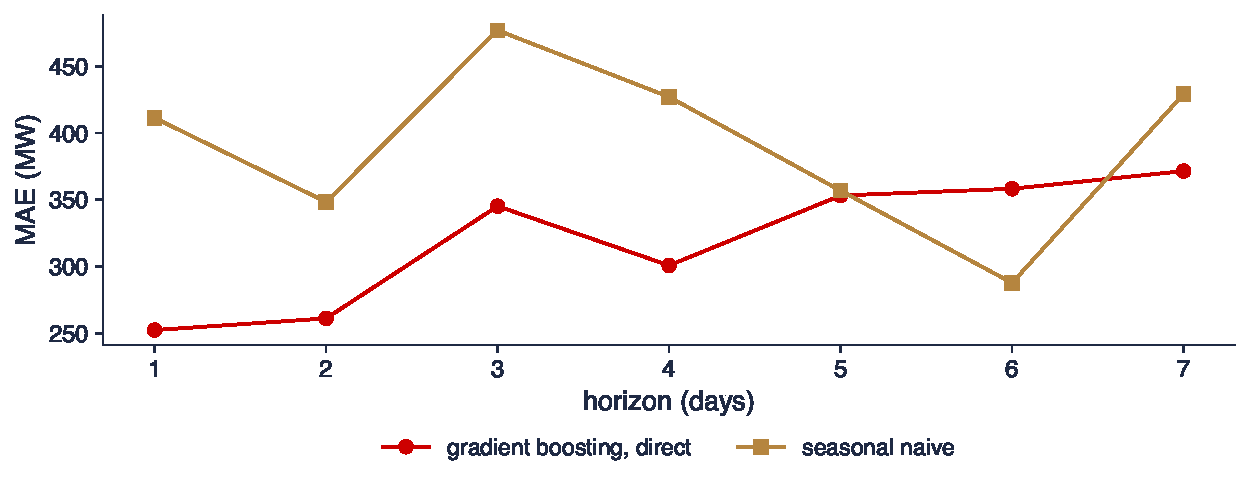
\includegraphics[width=0.96\textwidth,height=0.34\textheight,keepaspectratio]{ch9_sem_b1.pdf}
\end{center}
\vspace{-2mm}
\begin{itemize}
    \item 25 origins, 7 horizons; MAE: GB 320 MW, seasonal naive 391 MW; RMSE 409 and 521 MW; MASE 1.04 and 1.27 (scale 308 MW)
    \item DM (with the HLN correction) $= -2.63$, p 0.015; the worst origin for GB: 5 January 2026 (MAE 576 MW)
    \item Interpretation: one day ahead GB has 252 MW against 411 MW: it uses yesterday's level, which the seasonal naive ignores; at 7 days (371 and 429 MW) both rely on last week's pattern
\end{itemize}\quantlet{TSA\_ch9\_seminar}{\qlurl{TSA_ch9_seminar}}
\end{frame}

\begin{frame}{B2: recursive, direct and the value of holidays [Proposed]}
\itemsize{\footnotesize}
\begin{itemize}
\item \textbf{Question}: does the recursive strategy forecast as well as the direct one, and how much do the holiday features help?
\item \textbf{Inputs}: the data and origins of B1; model: B1
\item \textbf{Tasks}
\begin{enumerate}
    \item Repeat B1 with the recursive strategy (\texttt{forecast\_recursive}).
    \item Repeat the direct model without the three holiday features (easter, xmas, holiday).
    \item Report the MAE of the three models on all days, on the public-holiday days and on the other days.
    \item Interpretation: which feature group explains most of the difference, and on which days?
\end{enumerate}
\item \textbf{Report}: nine MAE values and one sentence
\item Notebook: section B2
\end{itemize}
\end{frame}

\ifsolutions
\begin{frame}{B2: solution [Proposed]}
\itemsize{\scriptsize}
\begin{center}
\includegraphics[width=0.96\textwidth,height=0.34\textheight,keepaspectratio]{ch9_sem_b2.pdf}
\end{center}
\vspace{-2mm}
\begin{itemize}
    \item MAE (MW): direct 320, recursive 327, direct without holidays 323
    \item On the 9 holiday days: 470, 409 and 496 MW; on the other days: 312, 323 and 313 MW
    \item Interpretation: removing the holiday flags raises the error on holidays (470 to 496 MW) and leaves the other days almost unchanged; holidays stay the hardest days for every model; recursive and direct differ little
\end{itemize}\quantlet{TSA\_ch9\_seminar}{\qlurl{TSA_ch9_seminar}}
\end{frame}
\fi

\begin{frame}{B3: Romanian inflation three months ahead [Solved]}
\itemsize{\footnotesize}
\begin{itemize}
\item \textbf{Question}: can machine learning forecast Romanian inflation three months ahead better than the random walk and a linear AR model?
\item \textbf{Inputs}: 12-month HICP inflation of 27 EU countries (Eurostat), monthly, 2005--2026
\item \textbf{Tasks}
\begin{enumerate}
    \item Build the features of each country (inflation lags, monthly changes, calendar month) and the target $\pi_{t+3} - \pi_t$ with \texttt{inflation\_frame}.
    \item Every January from 2016, refit AR, lasso, random forest and GB on Romania only, and a global GB on all countries; forecast every month of the year.
    \item Compute the RMSE of each model and its ratio to the random walk.
    \item Run the DM test for AR against RW and for the global against the local GB.
    \item Interpretation: what happened to all models in 2021--2023?
\end{enumerate}
\item \textbf{Report}: six RMSEs, two DM tests and one sentence
\item Notebook: section B3
\end{itemize}
\end{frame}

\begin{frame}{B3: solution [Solved]}
\itemsize{\scriptsize}
\begin{center}
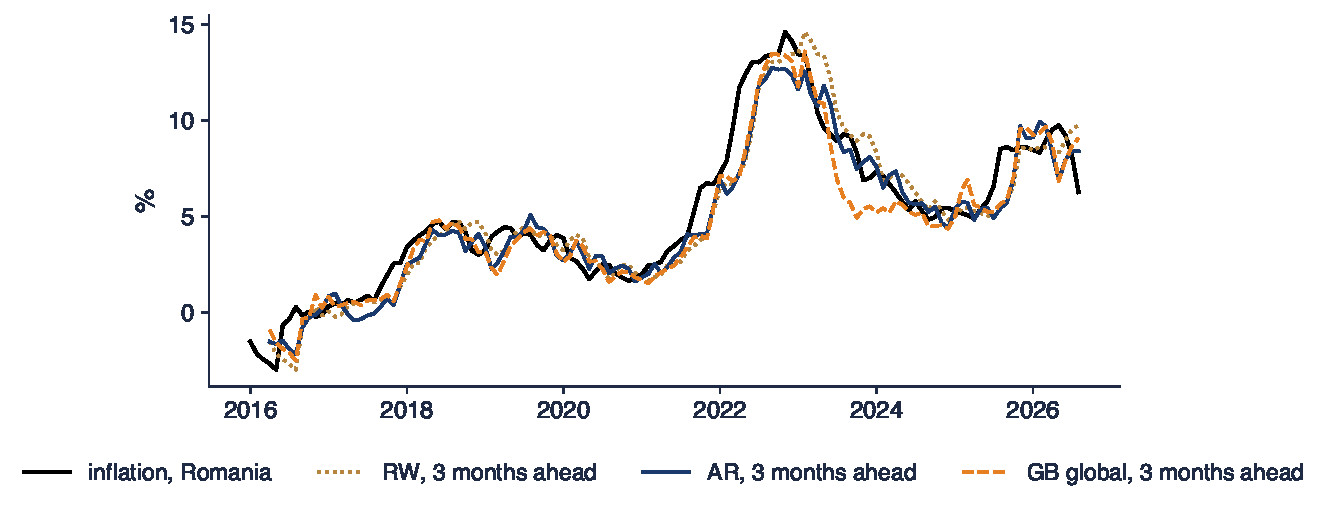
\includegraphics[width=0.96\textwidth,height=0.32\textheight,keepaspectratio]{ch9_sem_b3.pdf}
\end{center}
\vspace{-2mm}
\begin{itemize}
    \item 125 origins, January 2016--May 2026; RMSE (pp): RW 1.41, AR 1.28 (0.90), lasso 1.45 (1.02), RF 1.49 (1.06), GB local 1.64 (1.16), GB global 1.37 (0.97)
    \item DM: AR against RW $-1.33$ (p 0.186); GB global against GB local $-1.60$ (p 0.113)
    \item Interpretation: from mid-2021 to mid-2023 every RMSE jumps (RW 2.27, AR 2.02, GB global 2.09 pp): the energy shock was not in the past of inflation; pooling 27 countries helps the trees, but no model is significantly better than AR
\end{itemize}\quantlet{TSA\_ch9\_seminar}{\qlurl{TSA_ch9_seminar}}
\end{frame}

\begin{frame}{B4: the sign of BET returns [Proposed]}
\itemsize{\footnotesize}
\begin{itemize}
\item \textbf{Question}: can a classifier predict whether the BET rises tomorrow better than ``it always rises''?
\item \textbf{Inputs}: daily BET log returns since 2000; test years 2015--2026; model: B3 (yearly refits)
\item \textbf{Tasks}
\begin{enumerate}
    \item Build the features of \texttt{sign\_frame} (five lagged returns, sums over 5, 21, 63 days, volatility over 21 and 63 days) and the target $1\{r_{t+1} > 0\}$.
    \item Each January, fit a logistic regression and a gradient-boosting classifier on all earlier days; the baseline predicts the majority class of the training data.
    \item Report the accuracy of the three, the $z$ statistic against the baseline and the AUC.
    \item Interpretation: what does the result say about the weak-form efficiency of the Bucharest market?
\end{enumerate}
\item \textbf{Report}: three accuracies, two $z$ statistics, two AUCs and one sentence
\item Notebook: section B4
\end{itemize}
\end{frame}

\ifsolutions
\begin{frame}{B4: solution [Proposed]}
\itemsize{\scriptsize}
\begin{center}
\includegraphics[width=0.96\textwidth,height=0.32\textheight,keepaspectratio]{ch9_sem_b4.pdf}
\end{center}
\vspace{-2mm}
\begin{itemize}
    \item 2\,925 test days; up days 55.3\%; accuracy: baseline 55.3\%, logit 54.7\% ($z = -0.63$, p 0.527), GB 52.9\% ($z = -2.64$, p 0.008)
    \item AUC: logit 0.538, GB 0.528; the logit predicts ``up'' on 95.4\% of the days
    \item Interpretation: no gain over the baseline; the past returns carry almost no information about the next sign, as weak-form efficiency says
\end{itemize}\quantlet{TSA\_ch9\_seminar}{\qlurl{TSA_ch9_seminar}}
\end{frame}
\fi


%=============================================================================
\section{Part C: open questions and AI critique}
%=============================================================================

\begin{frame}{C1: a global model for European electricity load [Proposed]}
\itemsize{\footnotesize}
\begin{itemize}
    \item \textbf{Idea}: ENTSO-E publishes the hourly load of every European country; one global GB model trained on 20 countries may forecast Romania better than a local one
    \begin{itemize}
        \item features: lags scaled by each country's mean, weekday, national holidays, a country identifier
    \end{itemize}
    \item Questions to answer
    \begin{itemize}
        \item 1. Does the global model beat the local GB and DHR on the 26 origins of \tsachlink{https://danpele.github.io/Time-Series-Analysis/EN/Courses/chapter4_seasonality_forecasting.pdf}{Chapter 4}?
        \item 2. Does it forecast Orthodox Easter better, although most countries celebrate Western Easter?
        \item 3. Which countries help Romania most (leave-one-country-out)?
    \end{itemize}
    \item A possible team project: data, code, DM tests and a two-page report; model: B1, B3
\end{itemize}
\end{frame}

\begin{frame}{C2: audit an AI answer [Proposed]}
\itemsize{\scriptsize}
\begin{itemize}
    \item A student asked an AI assistant whether machine learning can forecast markets and electricity load. The answer:
    \item \aiprompt{(a) A random forest with 5-fold cross-validation explains 36.8\% of the next month's S\&P 500 return, so the market is predictable.}
    \item \aiprompt{(b) A logistic model predicts the daily sign with 53.8\% accuracy, well above 50\%: a profitable signal.}
    \item \aiprompt{(c) For the load, GB has MASE 0.97, so it is 3\% more accurate than DHR.}
    \item \aiprompt{(d) Standardise the whole series first, then split it into training and test.}
    \item \aiprompt{(e) An LSTM always beats ARIMA because it has long memory.}
    \item \aiprompt{(f) Calendar features of the target day, such as holidays, are allowed because they are known in advance.}
    \item Tasks
    \begin{itemize}
        \item 1. For each statement, say whether it is correct; if not, give the correct statement and, where possible, the correct number from the lecture notebook (sections 2, 6, 9).
        \item 2. Report: a list of six verdicts with one line of justification each.
    \end{itemize}
\end{itemize}
\end{frame}

\ifsolutions
\begin{frame}{C2: solution [Proposed]}
\itemsize{\scriptsize}
\begin{itemize}
    \item (a) Wrong: overlapping 21-day targets leak across shuffled folds; walk-forward gives $R^2$ = -38.6\%
    \item (b) Wrong: the baseline ``always up'' has 54.4\%; the model is below it
    \item (c) Wrong: MASE compares with the in-sample seasonal naive method, not with DHR; DHR has MASE 0.89, so GB is less accurate than DHR
    \item (d) Wrong: leakage; fit the scaler on each training window only
    \item (e) Wrong: on our load data the LSTM has MASE 1.16, worse than DHR, GB and ridge; M4: pure ML methods lost to simple combinations
    \item (f) Correct
\end{itemize}\quantlet{TSA\_ch9\_seminar}{\qlurl{TSA_ch9_seminar}}
\end{frame}
\fi


%=============================================================================
\section{Wrap-up}
%=============================================================================

\begin{frame}{Key takeaways}
\itemsize{\small}
\begin{itemize}
    \item A forecast is a prediction from features known at the origin: lags, past rolling means, calendar
    \item Recursive and direct strategies: compare them on the same origins
    \item Leakage: any value from after the origin, including through scaling or shuffled folds
    \item GB beats the seasonal naive forecast for the load; nothing beats ``always up'' for the sign of BET returns
    \item An AI answer is a draft: check the validation scheme and the benchmark behind every claimed accuracy
\end{itemize}
\end{frame}

\begin{frame}{After the seminar}
\itemsize{\small}
\begin{itemize}
    \item Lecture 9 develops each topic of today: features and strategies, walk-forward validation, ridge and lasso, trees and boosting, neural networks and the LSTM, prediction intervals, global models, the M4 and M5 competitions
    \item Try the [Proposed] tasks in the notebook
    \item C1 can grow into a team project: a global model for European electricity load
    \item Reading: \refHP, Ch.~10; \refFPP, Sec.~12.4; \refMMH
    \item \textbf{The seminar is for practice and is not graded; the solutions of [Proposed] tasks are discussed in class}
\end{itemize}
\end{frame}


%=============================================================================
\section{References}
%=============================================================================

\begin{frame}{References}
\itemsize{\tiny}
\begin{itemize}
    \item Diebold, F. X., \& Mariano, R. S. (1995). Comparing predictive accuracy. \textit{Journal of Business \& Economic Statistics}, 13(3), 253--263. \href{https://doi.org/10.1080/07350015.1995.10524599}{doi:10.1080/07350015.1995.10524599}
    \item Huang, C., \& Petukhina, A. (2022). \textit{Applied Time Series Analysis and Forecasting with Python}. Springer. \href{https://doi.org/10.1007/978-3-031-13584-2}{doi:10.1007/978-3-031-13584-2}
    \item Hyndman, R. J., \& Athanasopoulos, G. (2021). \textit{Forecasting: Principles and Practice} (3rd ed.), Section 12.4, Neural network models. OTexts. \href{https://otexts.com/fpp3/nnetar.html}{otexts.com/fpp3/nnetar.html}
    \item Hyndman, R. J., \& Koehler, A. B. (2006). Another look at measures of forecast accuracy. \textit{International Journal of Forecasting}, 22(4), 679--688. \href{https://doi.org/10.1016/j.ijforecast.2006.03.001}{doi:10.1016/j.ijforecast.2006.03.001}
    \item Kaufman, S., Rosset, S., Perlich, C., \& Stitelman, O. (2012). Leakage in data mining: Formulation, detection, and avoidance. \textit{ACM Transactions on Knowledge Discovery from Data}, 6(4), 1--21. \href{https://doi.org/10.1145/2382577.2382579}{doi:10.1145/2382577.2382579}
    \item Koenker, R., \& Bassett, G. (1978). Regression quantiles. \textit{Econometrica}, 46(1), 33--50. \href{https://doi.org/10.2307/1913643}{doi:10.2307/1913643}
    \item Lei, J., G'Sell, M., Rinaldo, A., Tibshirani, R. J., \& Wasserman, L. (2018). Distribution-free predictive inference for regression. \textit{Journal of the American Statistical Association}, 113(523), 1094--1111. \href{https://doi.org/10.1080/01621459.2017.1307116}{doi:10.1080/01621459.2017.1307116}
    \item Montero-Manso, P., \& Hyndman, R. J. (2021). Principles and algorithms for forecasting groups of time series: Locality and globality. \textit{International Journal of Forecasting}, 37(4), 1632--1653. \href{https://doi.org/10.1016/j.ijforecast.2021.03.004}{doi:10.1016/j.ijforecast.2021.03.004}
\end{itemize}
\end{frame}

\end{document}
